\section{Agate Fossil Beds National Monument}

\subsection{Current Grassland Management Goals and Programs}

\subsubsection{Grassland Management Goals}

The majority of management goals within Agate Fossil Beds National
Monument (AGFO) pertain to cultural resources management. The
Foundational Document and Resource Management Plan, focus on cultural
resource management and interpretation. Natural resources are not a
fundamental resource of value (FRV) for AGFO, nor are they mentioned to
any specifics in the enabling legislation of the unit. Interviews
conducted at AGFO stated the focus on cultural resources and simply
managing the prairie because it is included within the NPS property they
protect. The only goals were to maintain the prairie so that the
landscape could mimic what the area looked like when Red Cloud and James
Cook were present, and strive for invasive species eradication.

\subsubsection{Grassland Management Programs}

There are no continuous natural resource management efforts conducted by
unit staff as there are no natural resource staff stationed at the
monument.

\subsection{Management Plans and Data Available}

\subsubsection{Management Plans}

The Foundational Document, written in 2012, describes the prairie as an ``other important resource''. 
The Foundational Document states that the ``shortgrass prairie and the Niobrara riparian ecotone are regionally important parts of the high plains ecosystem.'' 
It gives no further ecological details. 
Management plans published in the last ten years are listed in Table~\ref{tab:AGFOManDocs}. 
The most recent, the Natural Resource Condition Assessment, was a useful resource in the completion of this report. 
The Foundation Statement was also beneficial as it laid out the goals and the main reasons for establishment of the monument. 
There are more management plans written, but they are over ten years old.
Effective adaptive management will likely require these older plans to be revisited and perhaps revised, particularly the 2001 fire management plan.

\begin{table}[h]
	\centering
\caption[AGFO management documents]
	{Management documents for AGFO published from 2008-2018} 
\label{tab:AGFOManDocs}
	\begin{tabular}{lc}
		\toprule
		Title & Year\tabularnewline
		\midrule
		Interpretive Plan & 2011 \tabularnewline
		Foundation Document & 2012 \tabularnewline
		Bison Reintroduction Feasibility & 2014 \tabularnewline
		Natural Resource Condition Assessment & 2018 \tabularnewline
		\bottomrule
	\end{tabular}
\end{table}

\subsubsection{Data Available}

Interviews expressed not much data is used or thought to exist at AGFO.
Monument staff interact with Northern Great Plains I\&M network professionals. 
It was stated several times that they rely on I\&M staff or other regional professional staff to alert to AGFO natural resource issues that arise. 
AGFO moved from the Heartland Monitoring Network to the Northern Great Plains Monitoring Network. 
This is the reason for two data sets of monitoring data.

\storeareas\normalsetting
\KOMAoption{paper}{landscape}
\areaset{1.5\textwidth}{.6\textheight}
\recalctypearea
\pagestyle{plain}
\setlength\LTcapwidth{1.5\textwidth} 
\setlength\LTleft{0pt}           
\begin{longtable}[l]{@{}p{5cm}p{2cm}p{3cm}p{4cm}p{3cm}p{4cm}p{3cm}@{}}
	\caption[AGFO data]
	{Selected data collected in AGFO, 2008-2018.} 
	\label{tab:AGFOdata} \\
	\toprule
	Data title & Data type & Spatial extent & Frequency & Duration & Collecting agency & Format located \tabularnewline
	\midrule
	\endfirsthead 
	\caption* {\textbf{Table \ref{tab:BADLdata}}, \emph{continued.}} \\
\toprule
Title of Data & Type of Data & Spatial Extent
& Frequency of Collection & Duration of
Collection & Collecting Agency & Format Located \tabularnewline
\midrule
\endhead
Climate Change Exposure & Climate & weather at the park unit & research
study & 1901-2012 & Monahan \& Fisichelli & IRMA\tabularnewline
Geologic Resources Inventory Report & Geology & park wide & inventory of
all available data on geology & summary of all park history up to 2009 &
NPS- Geologic Resources Division & IRMA\tabularnewline
Plant Community Composition & Vegetation & Unit wide & annually samples
6 plots & 2011- current & NPS- NGP I\&M & IRMA\tabularnewline
Plant Community Monitoring & Vegetation & 11 monitoring sites
established & each site sampled seven times & 1999-2009 & NPS- Heartland
Network I\&M & IRMA\tabularnewline
Riparian Invasive Plant & Vegetation & 48 2x2m plots in high yellow flag
iris wetland areas & 3 separate data collections & 2014-2015 & Thesis-
Colorado State University & IRMA\tabularnewline
Groundwater Monitoring & Water & three wells within the unit & pressure
and temperature recorded by data loggers at half-hour intervals &
2006-2010 & NPS-WRD & IRMA\tabularnewline
Nebraska Stream Biological Monitoring Program & Water & Niobrara River &
Began in 1997 and sampling was conducted on a five year cycle. &
2004-2008 & Nebraska Department of Environmental Quality & web
search\tabularnewline
Fish Inventory & Wildlife & 2,000m of Niobrara river electro fished &
over three days of June 2008 & 2008 & University of Nebraska- Lincoln &
IRMA\tabularnewline
Aquatic Invertebrate Community & Wildlife & 3 locations separated by 3km
along Niobrara river, samplers deployed monthly over the summer &
annually & 1996-2009 & NPS- Heartland Network I\&M & IRMA, (data sheets
for the study available on site)\tabularnewline
Aquatic Invertebrates & Wildlife & Three sampling points in the Niobrara
River across the unit & seven sampling frames per summer & 2010-2014 &
NGP- I\&M & IRMA\tabularnewline
Landbird Monitoring & Wildlife & 96 points surveyed across the unit
(geospatially displayed in report) & once per year & 2013-2016 & NGP-
I\&M & IRMA\tabularnewline
Acoustic Bat Surveys & Wildlife & 43 stations across the unit & 4-7
nights each year & 2014-2016 & NGP- I\&M & IRMA\tabularnewline
Fish of the Niobrara River & Wildlife & 8 locations within monument
boundaries & June 26-28, 2011 & 2011 & University of Nebraska- Omaha &
IRMA\tabularnewline
Status of Native Stream Fishes in Protected Areas of the Niobrara River
& Wildlife & Niobrara river within AGFO & Four times & 1979, 1989, 2008,
2011 & various & IRMA\tabularnewline
2010 Field Season Report Bird Monitoring at AGFO & Wildlife & 40 points
across the monument & one time study & May 18- June 23, 2010 & Rocky
Mountain Bird Observatory & IRMA\tabularnewline
\bottomrule
\end{longtable}
\clearpage
\normalsetting
\pagestyle{fancy} 

\subsection{Disturbance Regimes }

\subsubsection{Grazing }

Heavy levels of livestock grazing were present on monument lands from the late 1880's until monument authorization in 1965. 
Removal of grazing allows fuel loads to build up causing AGFO to be of high danger for extreme fire behavior. 
The Department of Interior initiative, ``Back Home on the Range'', communicated the importance of establishing native herbivores, and particularly bison herds, within NPS units in the Great Plains (Hardy \& Plumb, 2016). 
AGFO was selected as a possible unit for reintroduction. 
Due to surrounding land management, Monument staff seem to be more open to a livestock grazing program than bison grazing.

\begin{figure}
	\centering
	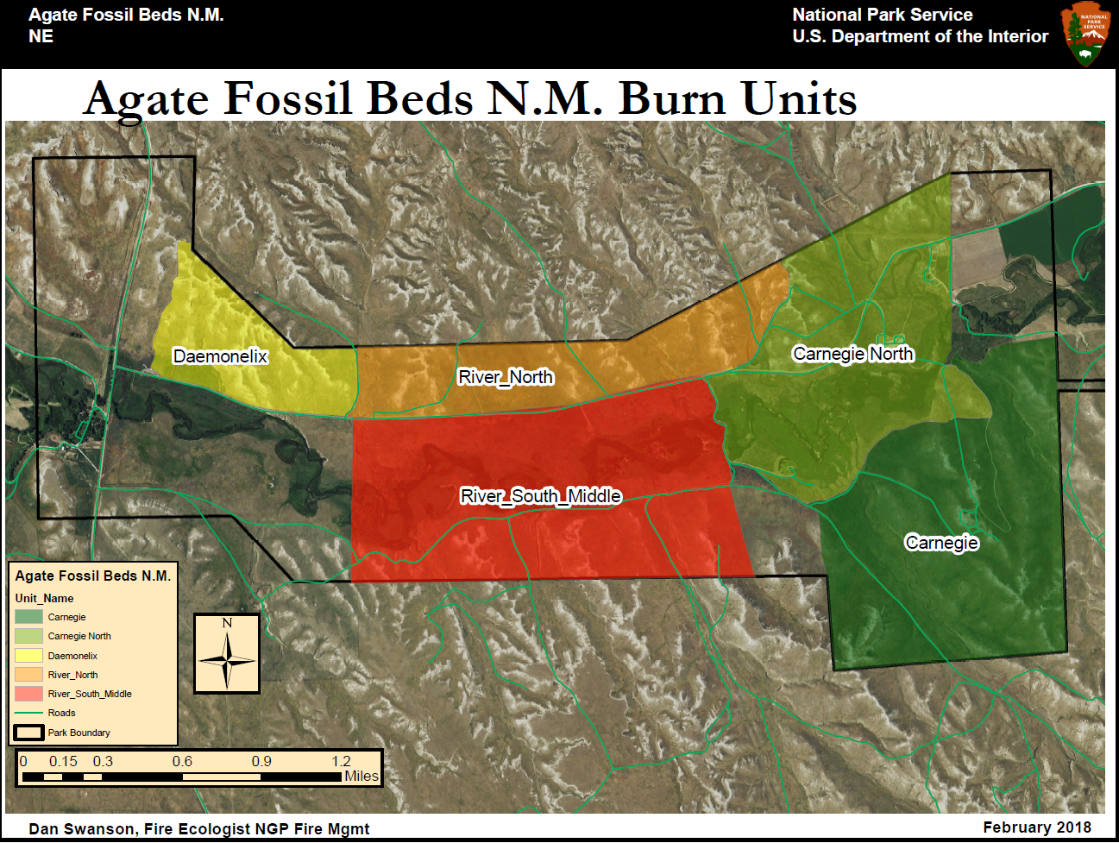
\includegraphics[width=5in,height=4in]{AGFO_Burn_Units}
	\caption{Burn units of AGFO}\label{fig:AGFOBurnUnits}
\end{figure}

\emph{Fire }

The 2001 Fire Management NEPA EA states, ``Park lands have not been grazed, burned (except for a few acres in a research project), or mowed (other than maintenance and thistle control) since the park's authorization.'' 
Since 2001, there has been some fire to create a burned
mosaic on the landscape (Fig.~\ref{fig:AGFOFireMosaic}). 
There are five burn units across the monument (Fig.~\ref{fig:AGFOBurnUnits}). 
Since 1992, there have been eight prescribed fires and two wildfires covering 1,907 acres.

\begin{figure} 
	\centering
	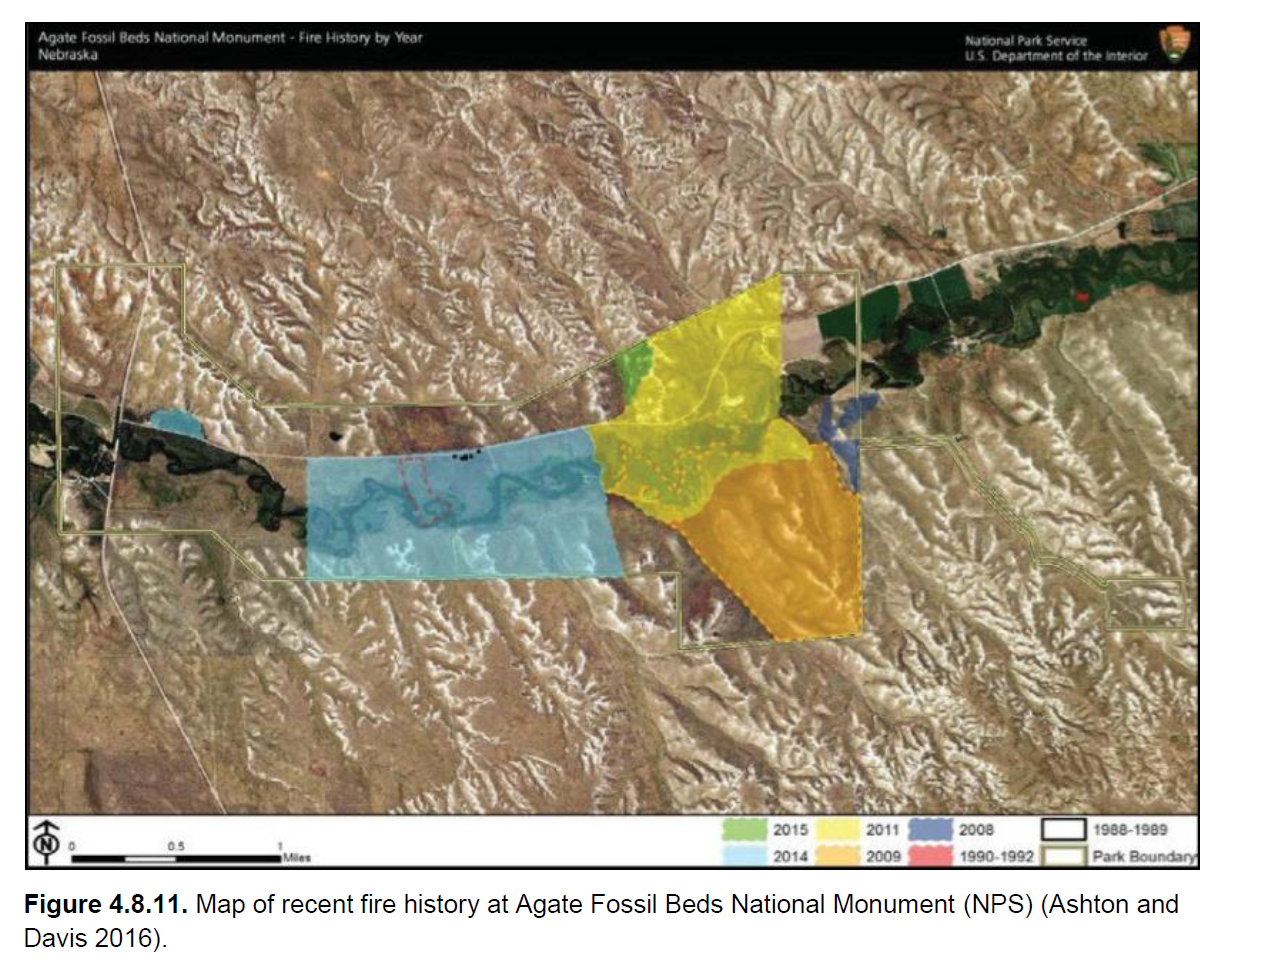
\includegraphics[width=6in,height=4.3in]{AGFO_Fire_Mosaic}
	\caption{Mosaic created through periodic burning at AGFO.} \label{fig:AGFOFireMosaic}
\end{figure}

\subsection{Data gaps and suggested research}

\subsubsection{Data Gaps}

Written documentation of landscape ecosystem goals would highly benefit the managers at AGFO. 
With little staff and scant funds to apply to natural resource management, having the most information available would allow them to best assign the resources they are allotted for the highest impact. 
Overall, there are data available from I\&M on vegetation and wildlife as well as extensive information on water quality and other aquatic resources. 
Using the data to implement some kind of management is the missing piece for AGFO. 
Although, as the landscape has not been disturbed significantly in recent years, the vegetative response to disturbance is a key data gap. 
Productivity data as well as erosion data is missing in terms of understanding the effect of a large grazer.
Livestock impact on the Niobrara River would be beneficial ahead of establishing a grazing disturbance.

\subsubsection{Suggested Research}

Of particular note was that during the interviews, Monument staff believe that a large grazer such as cattle may help to diminish their largest invasive species problem: the yellow flag iris. 
Repeated trampling by a large grazer seems to lessen populations of the invasive iris on surrounding lands (2016 Jordan Spark Study). 
There should be further research of grazing impacts on the AGFO prairie.

\subsection{Management Recommendations: Establish a grazer on the landscape}

With the significant lack of natural resources staff and a natural resources management program (and the goal of filling cultural positions ahead of natural resource positions), it would seem easier to enact a livestock grazing program than a bison grazing program. 
Although bison are the NPS preferred alternative, cattle can accomplish a similar goal with significantly less budgetary and staff input. 
To accomplish this, they may take suggestions from Tallgrass Prairie National Preserve who leases a pasture of their land to local cattle owners to manage the prairie to the most conservative AUM and seasonality of cattle grazing.
Cattle would also accomplish the cultural focus of the Monument in wanting to restore the prairie to what it looked like when James Cook and Red Cloud were living in the area.
Revenue from cattle grazing fees could be used to support cultural resource management. 
A focus would be put on restoring a grazer to the ecosystem while also increasing budgetary support to the true meaning of the Monument: cultural preservation.

Once the large grazer were established, fire should be more present on the landscape. 
It will aid in the movement of cattle across the unit. 
It is our recommendation that a coupled disturbance regime be established to increase heterogeneity of the grassland. 
Very little disturbance is currently present on the landscape. 
Introducing a coupled disturbance regime would benefit the wildlife that depend on this patch of habitat for their vitality.
